\runningheader{SAT Mathematics}{Nonlinear Equations and Systems}{Page \thepage\ of \numpages}

\begingradingrange{sat-nonlinear-eq}
\subsection*{Part I. Nonlinear equations in one variable}

\question[1]
The given equation relates the numbers $j, k$ and $m$. Which equation correctly expresses $k$ in terms of $j$ and $m$?
\[
14 j+5 k=m
\]

\begin{choices}
  \CorrectChoice $k=\frac{m-14 j}{5}$
  \choice $k=\frac{1}{5} m-14 j$
  \choice $k=\frac{14 j-m}{5}$
  \choice $k=5 m-14 j$
\end{choices}

\question[1]
In the given equation, $k$ is an integer constant. If the equation has no real solution, what is the least possible value of $k$?

\[
x(k x-56)=-16
\]

\begin{solutionorbox}[1in]
\end{solutionorbox}

\question[1]
What is the positive solution to the given equation?
\[
-4 x^{2}-7 x=-36
\]
\begin{choices}
  \choice $\frac{7}{4}$
  \CorrectChoice $\frac{9}{4}$
  \choice 4
  \choice 7
\end{choices}

\question[1]
The given equation relates the distinct positive real numbers $w, x$, and $y$. Which equation correctly expresses $w$ in terms of $x$ and $y$?
\[
\frac{14 x}{7 y}=2 \sqrt{w+19}
\]
\begin{choices}
  \choice $w=\sqrt{\frac{x}{y}}-19$
  \choice $w=\sqrt{\frac{28 x}{14 y}}-19$
  \CorrectChoice $w=\left(\frac{x}{y}\right)^{2}-19$
  \choice $w=\frac{x}{y}-19$
\end{choices}

\question[1]
Which of the following is a solution to the given equation?
\[
(x+2)(x+3)=(x-2)(x-3)+10
\]
\begin{choices}
  \CorrectChoice 1
  \choice 0
  \choice -2
  \choice -5
\end{choices}

\question[1]
In the equation above, $a$ is a constant and $a>0$. If the equation has two integer solutions, what is a possible value of $a$?

\[
x^{2}-a x+12=0
\]

\begin{solutionorbox}[1in]
\end{solutionorbox}

\question[1]
What is the solution set of the equation above?
\begin{choices}
  \choice $\{-1\}$
  \choice $\{5\}$
  \CorrectChoice $\{-1,5\}$
  \choice $\{0,-1,5\}$
\end{choices}

\newpage

\begin{center}
  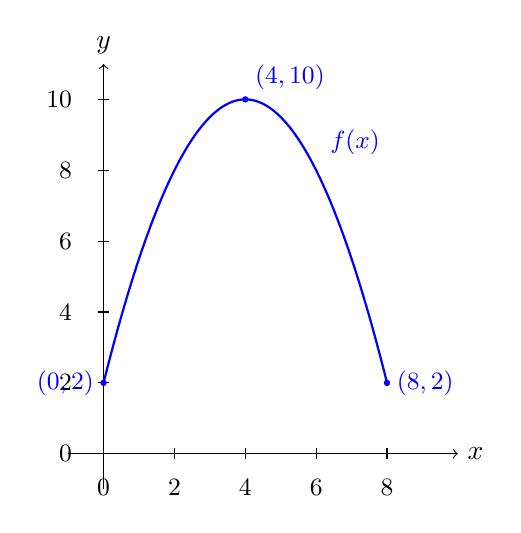
\begin{tikzpicture}[scale=0.45]
    % Axes
    \draw[->] (-1,0) -- (10,0) node[right] {$x$};
    \draw[->] (0,-1) -- (0,11) node[above] {$y$};
    \foreach \x in {0,2,4,6,8}
      \draw (\x,0.15) -- (\x,-0.15) node[below=4pt] {\small \x};
    \foreach \y in {0,2,4,6,8,10}
      \draw (0.15,\y) -- (-0.15,\y) node[left=6pt] {\small \y};

    % f(x) = -1/2(x-4)^2 + 10
    \draw[thick,blue,domain=0:8,samples=120]
      plot (\x,{-0.5*(\x-4)*(\x-4)+10});

    % Key points shown on the graph
    \filldraw[blue] (4,10) circle (2.1pt) node[above right] {\small $(4,10)$};
    \filldraw[blue] (0,2) circle (2.1pt) node[left] {\small $(0,2)$};
    \filldraw[blue] (8,2) circle (2.1pt) node[right] {\small $(8,2)$};
    \node[blue] at (7.1,8.8) {\small $f(x)$};
  \end{tikzpicture}
\end{center}

\question[1]
The graph of the function $f$, defined by $f(x)=-\frac{1}{2}(x-4)^{2}+10$, is shown in the $x y$-plane above. If the function $g$ (not shown) is defined by $g(x)=-x+10$, what is one possible value of $a$ such that $f(a)=g(a)$?

\begin{solutionorbox}[1in]
\end{solutionorbox}

\question[1]
In the given equation, $c$ is a constant. The equation has no real solutions if $c>n$. What is the least possible value of $n$?

\[
x^{2}-34 x+c=0
\]

\begin{solutionorbox}[1in]
\end{solutionorbox}

\question[1]
What is one possible solution to the given equation?

\[
|x-5|=10
\]

\begin{solutionorbox}[1in]
\end{solutionorbox}

\question[1]
In the given equation, $c$ is a constant. The equation has exactly one solution. What is the value of $c$?

\[
-16 x^{2}-8 x+c=0
\]

\begin{solutionorbox}[1in]
\end{solutionorbox}

\question[1]
What is the positive solution to the given equation?
\[
5 x^{2}-37 x-24=0
\]
\begin{choices}
  \choice $\frac{3}{5}$
  \choice 3
  \CorrectChoice 8
  \choice 37
\end{choices}

\question[1]
How many distinct real solutions does the given equation have?
\[
(x-1)^{2}=-4
\]
\begin{choices}
  \choice Exactly one
  \choice Exactly two
  \choice Infinitely many
  \CorrectChoice Zero
\end{choices}

\question[1]
What is one of the solutions to the given equation?

\[
z^{2}+10 z-24=0
\]

\begin{solutionorbox}[1in]
\end{solutionorbox}

\question[1]
How many distinct real solutions does the given equation have?
\[
5 x^{2}+10 x+16=0
\]
\begin{choices}
  \choice Exactly one
  \choice Exactly two
  \choice Infinitely many
  \CorrectChoice Zero
\end{choices}

\endgradingrange{sat-nonlinear-eq}

\newpage
\begingradingrange{sat-systems-eq}
\subsection*{Part II. Systems of equations in two variables}

\question[1]
If $\left(x_{1}, y_{1}\right)$ and $\left(x_{2}, y_{2}\right)$ are the two solutions to the system of equations above, what is the value of $y_{1}+y_{2}$?
\[
\begin{aligned}
& y=x^{2}+2 x+1 
& x+y+1=0
\end{aligned}
\]
\begin{choices}
  \choice -3
  \choice -2
  \choice -1
  \CorrectChoice 1
\end{choices}

\question[1]
If $u-3=\frac{6}{t-2}$, what is $t$ in terms of $u$?
\begin{choices}
  \choice $t=\frac{1}{u}$
  \choice $t=\frac{2 u+9}{u}$
  \choice $t=\frac{1}{u-3}$
  \CorrectChoice $t=\frac{2 u}{u-3}$
\end{choices}

\question[1]
In the given equation, $c$ is a constant. The equation has exactly one solution. What is the value of $c$?
\[
-9 x^{2}+30 x+c=0
\]
\begin{choices}
  \choice 3
  \choice 0
  \CorrectChoice -25
  \choice -53
\end{choices}

\question[1]
In the given equation, $c$ is a positive constant. Which of the following is one of the solutions to the given equation?
\[
\frac{x^{2}}{\sqrt{x^{2}-c^{2}}}=\frac{c^{2}}{\sqrt{x^{2}-c^{2}}}+39
\]
\begin{choices}
  \choice $-c$
  \choice $-c^{2}-39^{2}$
  \choice $-\sqrt{39^{2}-c^{2}}$
  \CorrectChoice $-\sqrt{c^{2}+39^{2}}$
\end{choices}

\question[1]
The given equation relates the distinct positive numbers $j, k$ and $m$. Which equation correctly expresses $j$ in terms of $k$ and $m$?
\[
8 j=k+15 m
\]
\begin{choices}
  \choice $j=\frac{k}{8}+15 m$
  \choice $j=k+\frac{15 m}{8}$
  \choice $j=8(k+15 m)$
  \CorrectChoice $j=\frac{k+15 m}{8}$
\end{choices}

\newpage

\question[1]
The graphs of the equations in the given system of equations intersect at the point $(x, y)$ in the $x y$-plane. What is a possible value of $x$?
\[
\begin{aligned}
& 8 x+y=-11 
& 2 x^{2}=y+341
\end{aligned}
\]
\begin{choices}
  \CorrectChoice -15
  \choice -11
  \choice 2
  \choice 8
\end{choices}

\question[1]
The speed of sound in dry air, $v$, can be modeled by the formula $v=331.3+0.606 T$, where $T$ is the temperature in degrees Celsius and $v$ is measured in meters per second. Which of the following correctly expresses $T$ in terms of $v$?
\begin{choices}
  \choice $T=\frac{v+0.606}{331.3}$
  \choice $T=\frac{v-0.606}{331.3}$
  \choice $T=\frac{v+331.3}{0.606}$
  \CorrectChoice $T=\frac{v-331.3}{0.606}$
\end{choices}

\question[1]
What is the sum of the solutions to the given equation?

\[
x(x+1)-56=4 x(x-7)
\]

\begin{solutionorbox}[1in]
\end{solutionorbox}

\question[1]
If $(x, y)$ is a solution to the system of equations above, which of the following is a possible value of $x$?
\[
\begin{aligned}
& x+y=12 
& y=x^{2}
\end{aligned}
\]
\begin{choices}
  \choice 0
  \choice 1
  \CorrectChoice 2
  \choice 3
\end{choices}

\question[1]
The given equation relates the numbers $p$ and $n$, where $n$ is not equal to 0 and $p>20$. Which equation correctly expresses $n$ in terms of $p$?
\[
p=20+\frac{16}{n}
\]
\begin{choices}
  \choice $n=\frac{p-20}{16}$
  \choice $n=\frac{p}{16}+20$
  \choice $n=\frac{p}{16}-20$
  \CorrectChoice $n=\frac{16}{p-20}$
\end{choices}

\question[1]
Which ordered pair $(x, y)$ is the solution to the given system of equations?
\[
\begin{gathered}
y=(x-2)(x+4) 
y=6 x-12
\end{gathered}
\]
\begin{choices}
  \choice $(0,2)$
  \choice $(-4,2)$
  \CorrectChoice $(2,0)$
  \choice $(2,-4)$
\end{choices}

\question[1]
The given equation relates the positive numbers $b, x$, and $y$. Which equation correctly expresses $x$ in terms of $b$ and $y$?
\[
\frac{1}{7 b}=\frac{11 x}{y}
\]
\begin{choices}
  \choice $x=\frac{7 b y}{11}$
  \choice $x=y-77 b$
  \CorrectChoice $x=\frac{y}{77 b}$
  \choice $x=77 b y$
\end{choices}

\question[1]
In the $x y$-plane, the graph of $y=x^{2}-9$ intersects line $p$ at $(1, a)$ and $(5, b)$, where $a$ and $b$ are constants. What is the slope of line $p$?
\begin{choices}
  \CorrectChoice 6
  \choice 2
  \choice -2
  \choice -6
\end{choices}

\question[1]
Blood volume, $V_B$, in a human can be determined using the equation $V_{B}=\frac{V_{P}}{1-H}$, where $V_{P}$ is the plasma volume and $H$ is the hematocrit (the fraction of blood volume that is red blood cells). Which of the following correctly expresses the hematocrit in terms of the blood volume and the plasma volume?
\begin{choices}
  \CorrectChoice $H=1-\frac{V_{P}}{V_{B}}$
  \choice $H=\frac{V_{B}}{V_{P}}$
  \choice $H=1+\frac{V_{B}}{V_{P}}$
  \choice $H=V_{B}-V_{P}$
\end{choices}

\newpage

\question[1]
What is the solution to the given equation?

\[
\frac{-54}{w}=6
\]

\begin{solutionorbox}[1in]
\end{solutionorbox}

\question[1]
The power $P$ produced by a machine is represented by the equation above, where $W$ is the work performed during an amount of time $t$. Which of the following correctly expresses $W$ in terms of $P$ and $t$?
\[
P=\frac{W}{t}
\]
\begin{choices}
  \CorrectChoice $W=P t$
  \choice $W=\frac{P}{t}$
  \choice $W=\frac{t}{P}$
  \choice $W=P+t$
\end{choices}

\question[1]
If one solution to the system of equations above is $(x, y)$, what is one possible value of $x$?

\[
\begin{array}{r}
x+y=17 
x y=72
\end{array}
\]

\begin{solutionorbox}[1in]
\end{solutionorbox}

\question[1]
The formula above can be used to approximate the dew point $D$, in degrees Fahrenheit, given the temperature $T$, in degrees Fahrenheit, and the relative humidity of $H$ percent, where $H>50$. Which of the following expresses the relative humidity in terms of the temperature and the dew point?
\[
D=T-\frac{9}{25}(100-H)
\]
\begin{choices}
  \CorrectChoice $H=\frac{25}{9}(D-T)+100$
  \choice $H=\frac{25}{9}(D-T)-100$
  \choice $H=\frac{25}{9}(D+T)+100$
  \choice $H=\frac{25}{9}(D+T)-100$
\end{choices}

\question[1]
Which of the following are solutions to the given equation, where $a$ is a constant and $a>30$?
\[
x-29=(x-a)(x-29)
\]
I. $a$
II. $a+1$
III. 29
\begin{choices}
  \choice I and II only
  \choice I and III only
  \CorrectChoice II and III only
  \choice I, II, and III
\end{choices}

\question[1]
In the given system of equations, $a$ is a constant. The graphs of the equations in the given system intersect at exactly one point, $(x, y)$, in the $x y$-plane. What is the value of $x$?
\[
\begin{gathered}
y=2 x^{2}-21 x+64 
y=3 x+a
\end{gathered}
\]
\begin{choices}
  \choice -8
  \choice -6
  \CorrectChoice 6
  \choice 8
\end{choices}

\question[1]
A solution to the given system of equations is $(x, y)$. Which of the following is a possible value of $x y$?
\[
\begin{aligned}
x^{2} & =6 x+y 
y & =-6 x+36
\end{aligned}
\]
\begin{choices}
  \CorrectChoice 0
  \choice 6
  \choice 12
  \choice 36
\end{choices}

\question[1]
If $a$ is a solution of the equation above and $a>0$, what is the value of $a$?

\[
x^{2}+x-12=0
\]

\begin{solutionorbox}[1in]
\end{solutionorbox}

\question[1]
In the $x y$-plane, the graph of $y=3 x^{2}-14 x$ intersects the graph of $y=x$ at the points $(0,0)$ and $(a, a)$. What is the value of $a$?

\begin{solutionorbox}[1in]
\end{solutionorbox}

\question[1]
Which ordered pair $(x, y)$ is a solution to the given system of equations?
\[
\begin{gathered}
x+7=10 
(x+7)^{2}=y
\end{gathered}
\]
\begin{choices}
  \choice $(3,100)$
  \choice $(3,3)$
  \CorrectChoice $(3,10)$
  \choice $(3,70)$
\end{choices}

\newpage

\question[1]
In a city, the property tax $T$, in dollars, is calculated using the formula above, where $P$ is the value of the property, in dollars. Which of the following expresses the value of the property in terms of the property tax?
\[
T=0.01(P-40,000)
\]
\begin{choices}
  \choice $P=100 T-400$
  \choice $P=100 T+400$
  \choice $P=100 T-40,000$
  \CorrectChoice $P=100 T+40,000$
\end{choices}

\question[1]
What is a solution to the given equation?
\[
\frac{x^{2}}{25}=36
\]
\begin{choices}
  \choice 6
  \CorrectChoice 30
  \choice 450
  \choice 900
\end{choices}

\question[1]
The formula above expresses the square of the speed $v$ of a wave moving along a string in terms of tension $T$, mass $m$, and length $L$ of the string. What is $T$ in terms of $m, v$, and $L$?
\[
v^{2}=\frac{L T}{m}
\]
\begin{choices}
  \CorrectChoice $T=\frac{m v^{2}}{L}$
  \choice $T=\frac{m}{v^{2} L}$
  \choice $T=\frac{m L}{v^{2}}$
  \choice $T=\frac{L}{m v^{2}}$
\end{choices}

\question[1]
In the given equation, $a$ and $b$ are positive constants. The sum of the solutions to the given equation is $k(4 a+b)$, where $k$ is a constant. What is the value of $k$?

\[
64 x^{2}-(16 a+4 b) x+a b=0
\]

\begin{solutionorbox}[1in]
\end{solutionorbox}

\question[1]
What is one possible solution to the given equation?

\[
|x-2|=9
\]

\begin{solutionorbox}[1in]
\end{solutionorbox}

\question[1]
If $(x, y)$ is a solution of the system of equations above and $x>0$, what is the value of $x y$?
\[
2 y+6=2(x+3)
\]
\begin{choices}
  \choice 1
  \choice 2
  \choice 3
  \choice 9
\end{choices}

\question[1]
What is the sum of the solutions to the given equation?
\[
x^{2}-40 x-10=0
\]
\begin{choices}
  \choice 0
  \choice 5
  \choice 10
  \CorrectChoice 40
\end{choices}

\question[1]
The graphs of the equations in the given system of equations intersect at the point $(x, y)$ in the $x y$-plane. What is the value of $y$?
\[
\begin{gathered}
x=8 
y=x^{2}+8
\end{gathered}
\]
\begin{choices}
  \choice 8
  \choice 24
  \choice 64
  \CorrectChoice 72
\end{choices}

\newpage

\question[1]
What is the positive solution to the given equation?

\[
\frac{55}{x+6}=x
\]

\begin{solutionorbox}[1in]
\end{solutionorbox}

\question[1]
How many solutions are there to the system of equations above?
\[
\begin{aligned}
& y=x^{2}+3 x-7 
& y-5 x+8=0
\end{aligned}
\]
\begin{choices}
  \choice There are exactly 4 solutions.
  \choice There are exactly 2 solutions.
  \CorrectChoice There is exactly 1 solution.
  \choice There are no solutions.
\end{choices}

\question[1]
What are the solutions to the given equation?
\[
6 x^{2}+5 x-7=0
\]
\begin{choices}
  \CorrectChoice $\frac{-5 \pm \sqrt{25+168}}{12}$
  \choice $\frac{-6 \pm \sqrt{25+168}}{12}$
  \choice $\frac{-5 \pm \sqrt{36-168}}{12}$
  \choice $\frac{-6 \pm \sqrt{36-168}}{12}$
\end{choices}

\question[1]
What value of $x$ satisfies the equation above?
\[
\frac{4 x^{2}}{x^{2}-9}-\frac{2 x}{x+3}=\frac{1}{x-3}
\]
\begin{choices}
  \choice -3
  \choice $-\frac{1}{2}$
  \CorrectChoice $\frac{1}{2}$
  \choice 3
\end{choices}

\question[1]
In the given equation, $b$ is a constant. For which of the following values of $b$ will the equation have more than one real solution?
\[
64 x^{2}+b x+25=0
\]
\begin{choices}
  \CorrectChoice -91
  \choice -80
  \choice 5
  \choice 40
\end{choices}

\question[1]
Which of the following values of $x$ satisfies the given equation?
\[
x^{2}=64
\]
\begin{choices}
  \CorrectChoice -8
  \choice 4
  \choice 32
  \choice 128
\end{choices}

\question[1]
The solution to the given system of equations is $(x, y)$. What is the value of $y$?

\[
\begin{gathered}
y=x^{2}+14 x+48 
x+8=11
\end{gathered}
\]

\begin{solutionorbox}[1in]
\end{solutionorbox}

\question[1]
The total revenue from sales of a product can be calculated using the formula $T=PQ$, where $T$ is the total revenue, $P$ is the price of the product, and $Q$ is the quantity of the product sold. Which of the following equations gives the quantity of product sold in terms of $P$ and $T$?
\begin{choices}
  \choice $Q=\frac{P}{T}$
  \CorrectChoice $Q=\frac{T}{P}$
  \choice $Q=P T$
  \choice $Q=T-P$
\end{choices}

\question[1]
In the given system of equations, $a$ is a positive constant. The system has exactly one distinct real solution. What is the value of $a$?

\[
\begin{gathered}
y=-1.50 
y=x^{2}+8 x+a
\end{gathered}
\]

\begin{solutionorbox}[1in]
\end{solutionorbox}

\question[1]
When the equations above are graphed in the $x y$-plane, what are the coordinates $(x, y)$ of the points of intersection of the two graphs?
\[
\begin{aligned}
& y=x^{2}-1 
& y=3
\end{aligned}
\]
\begin{choices}
  \CorrectChoice $(2,3)$ and $(-2,3)$
  \choice $(2,4)$ and $(-2,4)$
  \choice $(3,8)$ and $(-3,8)$
  \choice $(\sqrt{2}, 3)$ and $(-\sqrt{2}, 3)$
\end{choices}

\question[1]
If $|4 x-4|=112$, what is the positive value of $x-1$?

\begin{solutionorbox}[1in]
\end{solutionorbox}

\question[1]
In the $x y$-plane, the graph of the equation $y=-x^{2}+9 x-100$ intersects the line $y=c$ at exactly one point. What is the value of $c$?
\begin{choices}
  \choice $-\frac{481}{4}$
  \choice -100
  \CorrectChoice $-\frac{319}{4}$
  \choice $-\frac{9}{2}$
\end{choices}

\question[1]
The given equation relates the positive numbers $b, c$, and $f$. Which equation correctly expresses $c$ in terms of $b$ and $f$?
\[
b=42 c f
\]
\begin{choices}
  \CorrectChoice $c=\frac{b}{42 f}$
  \choice $c=\frac{b-42}{f}$
  \choice $c=42 b f$
  \choice $c=42-b-f$
\end{choices}

\newpage

\question[1]
If $(x+5)^{2}=4$, which of the following is a possible value of $x$?
\begin{choices}
  \choice 1
  \choice -1
  \choice -2
  \CorrectChoice -3
\end{choices}

\question[1]
What is the negative solution to the given equation?

\[
38 x^{2}=38(9)
\]

\begin{solutionorbox}[1in]
\end{solutionorbox}

\question[1]
In the equation above, $a$ and $c$ are positive constants. How many times does the graph of the equation above intersect the graph of the equation $y=a+c$ in the $x y$-plane?
\[
y=a x^{2}-c
\]
\begin{choices}
  \choice Zero
  \choice One
  \CorrectChoice Two
  \choice More than two
\end{choices}

\question[1]
What value of $x$ satisfies the equation above?

\[
\sqrt{x+4}=11
\]

\begin{solutionorbox}[1in]
\end{solutionorbox}

\question[1]
The solution to the given system of equations is $(x, y)$. What is the value of $x$?

\[
\begin{gathered}
x^{2}+y+7=7 
20 x+100-y=0
\end{gathered}
\]

\begin{solutionorbox}[1in]
\end{solutionorbox}


\endgradingrange{sat-systems-eq}